\section{Kurven}
\begin{itemize}
\item Parameterform (Vektorform) $\vec{c}=\vec{\gamma}$ Intervall$\rightarrow\R^n$ $(nD)$
\begin{align*}
	\vec{c}=\begin{pmatrix}x(t) \\y(t)\\\vdots\end{pmatrix} \text{ bzw. } \begin{pmatrix}\varphi(t) \\\psi(t)\\\vdots\end{pmatrix}
\end{align*}
\item Explizite Darstellung $y=f(x)$ \\
	Durch Parameterelimination erhält man aus der Parameterform die Explizite Darstellung
\item Implizite Gleichung in $x,y\quad (x,y\in \text{Intervall})$
\end{itemize}
Umformung: Parameterform $\rightarrow$ Explizite Form $\rightarrow$ Implizite Form, Eine Umkehrung kann, muss aber nicht existieren. 

\subsection{Tangentialvektor}
\begin{align*}
\vec{c}'(t)&=(x'(t);y'(t)) \quad 2D\\
\vec{c}'(t)&=(x'(t);y'(t);z'(t)) \quad 3D\\
\abs{\vec{c}}&= \sqrt{x'^2+ y'^2+\dots} \text{Länge des Tangentialvektors} 
\end{align*}

\subsection{Kegelschnitte}
% TODO

\subsection{p.m. Tangentengleichung}
$f'(x) =\frac{\mathrm{d}f}{\dx}=\frac{\mathrm{d}y}{\dx}$\\
Tangentengleichung am Punkt $P=(x_0,y_0)$:
\begin{align*}
	y=y_0+f'(x_0)(x-x_0)
\end{align*}

\subsection{Implizit Ableiten}
Ableiten ohne Funktion:
\begin{enumerate}
\item Gleichung beidseitig differenzieren (d*)
\item mit bekannten Regeln nach Funktionsvariablen ableiten (Linearität, Produkt, Quotient)
\item Division durch $\dx$
\item nach $\frac{\mathrm{d}y}{\dx}$ Auflösen
\end{enumerate}

\subsection{Normale}
Gerade die senkrecht von der Funktion weg zeigt.
\[
y = y_0{\color{red}-}\frac{1}{f'(x_0)}(x-x_0)
\]

\subsection{Anstiegsformel (Tangentialsteigung)}
\[
f'(x)=\frac{\dy}{\dx}=\frac{y'(t)\dt}{x'(t)\dt}=\frac{y'(t)}{x'(t)}
\]
$\dt$ kann gekürzt werden

\subsection{Polarkoordinaten}
\begin{itemize}
\item Pol $=$ Zentrum
\item Polrichtung $= 0^{\circ}$-Richtung
\item Radius $=$ Formel von $\varphi$\\
$\varphi = $ Polarwinkel (\kom{gegen den Uhrzeigersinn})
\end{itemize}

\begin{itemize}
\item $r-\phi$-Diagram ($r$ als Funktion von $\phi$ mit $r\leq 0$)
\begin{center}
    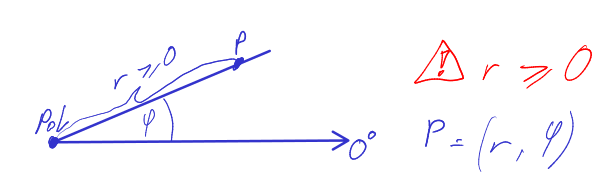
\includegraphics[height=2cm]{graphics/r-phi-graph.png}
\end{center}
\end{itemize}

